%
% File dialbot.tex
%
%% Based on the style files for ACL 2020, which were
%% Based on the style files for ACL 2018, NAACL 2018/19, which were
%% Based on the style files for ACL-2015, with some improvements
%%  taken from the NAACL-2016 style
%% Based on the style files for ACL-2014, which were, in turn,
%% based on ACL-2013, ACL-2012, ACL-2011, ACL-2010, ACL-IJCNLP-2009,
%% EACL-2009, IJCNLP-2008...
%% Based on the style files for EACL 2006 by 
%%e.agirre@ehu.es or Sergi.Balari@uab.es
%% and that of ACL 08 by Joakim Nivre and Noah Smith

\documentclass[11pt,a4paper]{article}
\usepackage[hyperref]{acl2020}
\usepackage{times}
\usepackage{latexsym}
\usepackage{amsmath} 
\renewcommand{\UrlFont}{\ttfamily\small}
\usepackage[T1]{fontenc}
% This is not strictly necessary, and may be commented out,
% but it will improve the layout of the manuscript,
% and will typically save some space.
\usepackage{microtype}

\aclfinalcopy % Uncomment this line for the final submission
%\def\aclpaperid{***} %  Enter the acl Paper ID here

%\setlength\titlebox{5cm}
% You can expand the titlebox if you need extra space
% to show all the authors. Please do not make the titlebox
% smaller than 5cm (the original size); we will check this
% in the camera-ready version and ask you to change it back.

\newcommand\BibTeX{B\textsc{ib}\TeX}

\title{Dialbot: muturretik muturrerako dialogo sistema}

\author{Julen Etxaniz \\
  University of the Basque Country \\
  jetxaniz007@ikasle.ehu.eus \\\And
  Aitor Zubillaga \\
  University of the Basque Country \\
  azubillaga012@ikasle.ehu.eus \\}

\date{}

\usepackage{graphicx}
\graphicspath{ {../images/} }
\begin{document}

\maketitle

\begin{abstract}
Proiektu honetan ikasketa sakonean oinarritutako muturretik muturrerako dialogo sistema bat garatu da itzulpenerako eredu bat eta pelikuletako azpitituluak erabiliz. Ingeleseko eredua ulertu eta probatu dugu eta euskararako bi eredu entrenatu ditugu, bat testuingururik gabea eta bestea testuinguruduna. Ereduen eskuzko ebaluazioa egin dugu eta metrika automatikoak ere kalkulatu ditugu. Kontuan hartuta dialogoa ez dela itzulpeneko ataza bat, emaitzak onargarriak direla esan dezakegu. Bukatzeko, sistema guztia telegrameko bot bezala funtzionatzeko egokitu dugu.
\end{abstract}

\section{Sarrera}

Proiektu honetan ikasketa sakonean oinarritutako muturretik muturrerako solasaldi sistema bat garatu da \citep{bahdanau2014neural} lanean oinarritua eta filmetako azpitituluak erabiliz \citep{lison2016opensubtitles2016}. Honetarako, dialogoa itzulpen ataza bat bezala proposatu da, hurrengo adibidean ikus daitekeen bezala:

\begin{itemize}
   \item Itzulpen automatikoa:
   \begin{itemize}
     \item Sistemaren sarrera - esaldia jatorri hizkuntza batean: "Egun on guztioi."
     \item Sistemaren irteera - esaldia helburu hizkuntzan: "Buenos días a todos."
   \end{itemize}
   \item Dialogoa:
   \begin{itemize}
     \item Sistemaren sarrera - dialogoko partaide baten esaldia: "Egun on guztioi."
     \item Sistemaren irteera - sarrerako esaldiari erantzuna: "Baita zuri ere."
   \end{itemize}
\end{itemize}

\section{Helburuak}

Proiektu honen helburuak honakoak dira:
\begin{enumerate}
    \item Ingeleserako entrenatua izan den muturretik muturrerako
solasaldi sistemaren eredua deskargatu eta probatzea. Honetaz gain, sistemaren arkitektura eta entrenamendurako erabilitako datuak aztertzea.

\item Euskarazko filmen azpitituluekin eredu berri bat entrenatzea.

\item Telegrameko bot bat sortzea, aurretik aipatutako bi ereduak integratzen dituena.

\item  Aurreko txandako galdera kontuan erabilita dialogoaren testuingurua kontuan hartzen duen sistema berri bat garatzea.

\end{enumerate}

\section{Erlazionatutako lanak}

Proiektu honetan ikasketa sakonean oinarritutako muturretik muturrerako solasaldi sistema bat garatu da \citep{bahdanau2014neural} lanean oinarritua eta filmetako azpitituluak erabiliz \citep{lison2016opensubtitles2016}. Hiztegia sortzeko Byte Pair Encoding (BPE) algoritmoa erabili dugu \citep{sennrich2015neural}.

Oinarri moduan irakasleak emandako  \href{https://drive.google.com/drive/folders/1a6JIZ96fupi8gHxYf5ytgkBc9zenJtQU}{kodea} erabili dugu. Bertan ingeleserako entrenatutako eredua dago. Gainera, ingeleseko sistema entrenatzeko erabili diren datuak eta kodea daude.

Gure kodea hedatzeko baliabide gehiago erabili ditugu. Alde batetik, Pytorch-eko tutorialak erabili dira. Bestetik, Ben Trevett-en tutorialak ere erabilgarriak izan dira.

\section{Datuak}

Esan bezala, filmetako azpitituluak erabiliko ditugu gure ereduak entrenatzeko. Hurrengo helbidean hizkuntza askotako azpititulu fitxategiak dituzu: \href{http://opus.nlpl.eu/OpenSubtitles-v2018.php}{http://opus.nlpl.eu/OpenSubtitles-v2018.php}. Ereduak entrenatzeko erabili den euskarazko fitxategia \href{http://opus.nlpl.eu/download.php?f=OpenSubtitles/v2018/mono/OpenSubtitles.raw.eu.gz}{hemen} aurki daiteke. Fitxategi honek milioi bat lerro inguru ditu. Lerro bakoitzean dialogoko partaide batek esaten duena dago.

Datuak filmetako azpitituluak izateak ereduak ikasi dezakeena baldintzatzen du. Horregatik, ingeleseko eredua entrenatzeko beste datu batzuk erabili dira, pertsonen arteko elkarrizketak. Euskararako aukera hori egongo balitz seguruenik hobea izango litzeteke.

\section{Sistema}

\subsection{Aurreprozesamendua}

Sarea entrenatu ahal izateko euskarazko dataseta ingelesekoaren formatu berdinean jarri dugu.

Hasteko, \texttt{eu.txt} fitxategiko 500.000 lerro irakurriko ditugu. Ondoren, lerro bakoitza garbituko dugu, letrak eta \texttt{.?!} puntuazio ikurrak bakarrik utziz. Gero, testua tokenizatuko dugu, esaldiko tokenak espazio batekin banatuz. Jarraian, sarrera eta irteera pareak osatuko ditugu \texttt{\t} ikurrarekin banatuz. Amaitzeko, \texttt{eu.tsv} fitxategian gordeko dugu dialogoa. 

Testuingurua kontuan hartzeko, dialogoko aurreko interakzioa ere kontuan hartuko dugu. Beraz, sarreran 3 esaldi egongo dira, eta irteeran bat. Kasu honetan 100.000 lerro irakurri ditugu. Dialogo hau \texttt{eu\_context.tsv} fitxategian gordeko dugu. Hona hemen testuinguruaren adibide bat: 

\begin{enumerate}
\item Txanda:
    \begin{itemize}
    \item Erabiltzailea: Kaixo.
    \item Sistema:
        \begin{itemize}
        \item Input -> Kaixo
        \item Output -> Kaixo
        \end{itemize}
    \end{itemize}
\item Txanda:
    \begin{itemize}
    \item Erabiltzailea: Zer moduz?
    \item Sistema:
        \begin{itemize}
        \item Input -> Kaixo Kaixo Zer moduz?
        \item Output -> Ondo eta zu?
        \end{itemize}
    \end{itemize}
\item Txanda
    \begin{itemize}
    \item Erabiltzailea: Ni ere
    \item Sistema:
        \begin{itemize}
        \item Input -> Zer moduz? Ondo eta zu? Ni ere
        \item Output -> Pozten naiz.
        \end{itemize}
    \end{itemize}
\end{enumerate}

Ingeleseko ereduan entrenamendurako datuak bakarrik erabili dira. Guk datuak hiru multzotan banatzea erabaki dugu, entrenamendua, balidazioa eta proba. Horrela, entrenatzen ari garen bitartean balidazioko datuetan probatu ahal izango dugu. Ondoren, probako datuak erabili ditzakegu emaitzak ikusteko. Datuen banaketa ausaz egin dugu, hurrengo tamainak erabiliz: entrenamendurako \%80, balidaziorako \%10 eta probarako \%10.

\subsection{Tokenizatzailea}

Hiztegia sortu dugu Byte Pair Encoding (BPE) algoritmoa erabiliz \citep{sennrich2015neural}. Defektuz 10000 subtoken definituko ditugu. Itzulpen automatiko neuronaleko ereduek hiztegi finkoarekin funtzionatzen dute normalean, baina itzulpena hiztegi irekiko arazoa da. Artikulu honetan, eredua hiztegi irekiko itzulpena egiteko gai da, hitz arraroak eta ezezagunak azpihitz unitateen kodifikatuz sekuentzia gisa.

Tokenizatzeko sarrera moduan aurreprozesatutako fitxategi osoa erabili dugu. Atzera begira, agian zentzu gehiago edukiko luke entrenamenturako datuak bakarrik erabiltzeak. Bestela, balidazioko eta probako datuak erabiltzen ari gara entrenamenduan eta horrek ereduari abantaila ematen dio. Horretarako, datuak tokenizatu aurretik banatu beharko lirateke, eta ondorekin hiru multzoak tokenizatu.

\subsection{Eredua}

Muturretik muturrerako sistema hau \citep{bahdanau2014neural} artikuluan proposatutako sisteman oinarritzen da. Hau itzulpen automatikoko sistema bat da, beraz, dialogoa itzulpen automatikoko ataza bat bezala definitzen ari gara. Aukera hau ez da optimoa sinplifikazio handi bat baita, hala ere, esperimentu interesgarriak egiteko aukera ematen digu.

\subsubsection{Seq2Seq}
Sekuentziatik sekuentziarako eredu (seq2seq) ohikoenak kodetzaile-deskodetzaile ereduak dira. Normalean sare errekurrente neuronal bat (RNN) erabiltzen dute sarrerako esaldia testuinguru bektorean kodetzeko. Bektore hau sarrerako esaldi osoaren errepresentazio abstraktua dela esan dezakegu. Bektore hau bigarren RNN batek deskodetzen du eta horrek irteerako esaldia ikasten du hitzak banaka sortuz.

Adibidez, ikusi \ref{fig:seq2seq} irudia. Sarrera esaldia, "guten morgen", embedding geruzatik (horia) igarotzen da eta ondoren kodetzailean sartzen da (berdea). Halaber, sekuentzia hasiera \texttt{<sos>} eta sekuentziaren amaiera \texttt{<eos>} tokenak eransten ditugu. Adibide honetan $X = \{x_1, x_2, ..., x_T\}$ daukagu, non $x_1 = \text{<sos>}, x_2 = \text{guten}$, etab. Hasierako egoera ezkutua, $h_0$, normalean zerora hasieratzen da edo ikasitako parametro batera.

Urrats bakoitzean, RNN kodetzailearen sarrera uneko hitzaren embeddinga txartatzen da, $e(x_t)$, baita aurreko denbora-urratsaren ezkutuko egoera ere, $h_{t-1}$, eta RNN kodetzaileak ezkutuko egoera berria ematen du $h_t$. Ezkutuko egoera orain arteko esaldiaren irudikapen bektorial gisa har dezakegu. Kodetzailea horrela erreperesenta daiteke:

$$h_t = \text{EncoderRNN}(e(x_t), h_{t-1})$$

Orain gure testuinguru bektorea dugu, $z$, deskodetzen has gaitezke irteerako esaldia lortzeko, "good morning". Berriro ere, hasierako eta bukaerako tokenak gehitzen dizkiogu esaldiari. Urrats bakoitzean, RNN deskodetzailearen sarrera (urdina) uneko hitzaren embeddinga, $d(y_t)$ da, baita aurreko urratsaren egoera ezkutua ere, $s_{t-1}$. Hasierako deskodetzailearen ezkutuko egoera, $s_0$, testuinguru bektorea da, $s_0 = z = h_T$. Horrela, kodetzailearen antzera, deskodetzailea honela irudika dezakegu:

$$s_t = \text{DecoderRNN}(d(y_t), s_{t-1})$$

Deskodetzailearen hitzak bata bestearen atzetik sortzen dira beti. Beti \texttt{<sos>} erabiltzen dugu deskodetzailearen lehen sarrerarako, $y_1$. Ondorengo sarreretarako, $y_{t>1}$, batzuetan sekuentziako eagiazko hurrengo hitza erabiliko dugu, $y_t$ eta batzuetan gure deskodetzaileak iragarritako hitza, $\hat{y}_{t-1}$. Honi teacher forcing deitzen zaio.

Gure eredua entrenatzerakoan edo probatzerakoan, badakigu zenbat hitz dauden helburuko esaldian, eta hitzak sortzeari uzten diogu. Inferentzian ohikoa da hitzak sortzen jarraitzea ereduak \texttt{<eos>} token bat itzuli arte edo hitz kopuru maximo batera iritsitakoan.

Aurreikusitako esaldia daukagunean, $\hat{Y} = \{ \hat{y}_1, \hat{y}_2, ..., \hat{y}_T \}$, helburuko esaldiarekin konparatzen dugu, $Y = \{ y_1, y_2, ..., y_T \}$, , galera kalkulatzeko. Ondoren, galera hori gure ereduko parametroak eguneratzeko erabiltzen dugu.

\begin{figure}[ht]
    \centering
    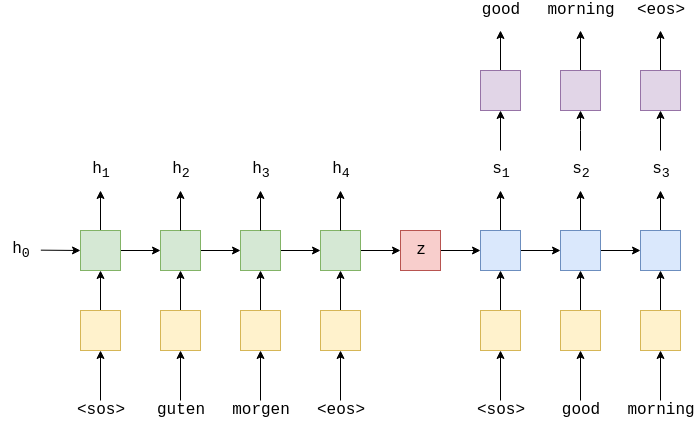
\includegraphics[width=\linewidth]{seq2seq}
    \caption{Eredua}
    \label{fig:seq2seq}
\end{figure}

\subsubsection{Kodetzailea}

RNN bidirekzionala erabiltzen dugu, geruza bakarreko GRU bat. Geruza bakoitzean bi RNN ditugu. Aurreranzko RNNtik esaldia ezkerretik eskuinera pasatuko da (berdez), eta atzeratutako RNNtik eskuinetik ezkerrera (urdinez). Ikusi \ref{fig:encoder} irudia. Hau horrela adieraz dezakegu:

$h_t^\rightarrow = \text{EncoderGRU}^\rightarrow(e(x_t^\rightarrow),h_{t-1}^\rightarrow)$

$h_t^\leftarrow = \text{EncoderGRU}^\leftarrow(e(x_t^\leftarrow),h_{t-1}^\leftarrow)$

non $x_0^\rightarrow = \text{\textless sos\textgreater}, x_1^\rightarrow = \text{guten}$ eta $x_0^\leftarrow = \text{\textless eos\textgreater}, x_1^\leftarrow = \text{morgen}$.

Hasierako aurreranzko eta atzeranzko ezkutuko egoerak izango ditugu ($h_0^\rightarrow$ eta $ h_0^\leftarrow$, hurrenez hurren). Bi testuinguru bektore ere lortuko ditugu, bata RNN aurreratua esaldian azken hitza ikusi ondoren, $z^\rightarrow=h_T^\rightarrow$, eta bestea RNN atzerakoia lehenengo hitza ikusi ondoren esaldian, $z^\leftarrow=h_T^\leftarrow$.

Aurreranzko eta atzeranzko ezkutuko egoerak konkatenatu ditzakegu, hau da, $h_1 = [h_1^\rightarrow; h_{T}^\leftarrow]$, $h_2 = [h_2^\rightarrow; h_{T-1}^\leftarrow]$. Egoera ezkutu guztiak horrela adieraz ditzakegu: $H=\{ h_1, h_2, ..., h_T\}$.

Deskodetzailea ez denez bidirekziola bektore bakarra behar du, $z$, hasierako ezkutuko egoera gisa erabiltzeko, $s_0$. deskodetzailean bi ditugu, $z^\rightarrow=h_T^\rightarrow$ eta $z^\leftarrow=h_T^\leftarrow$. Hau konpontzeko, bi testuinguru bektoreak elkarrekin kateatu, $g$ geruza lineal batetik pasatu eta $\tanh$ aktibazio funtzioa aplikatu dezakegu.

$$z=\tanh(g(h_T^\rightarrow, h_T^\leftarrow)) = \tanh(g(z^\rightarrow, z^\leftarrow)) = s_0$$

\begin{figure}[ht]
    \centering
    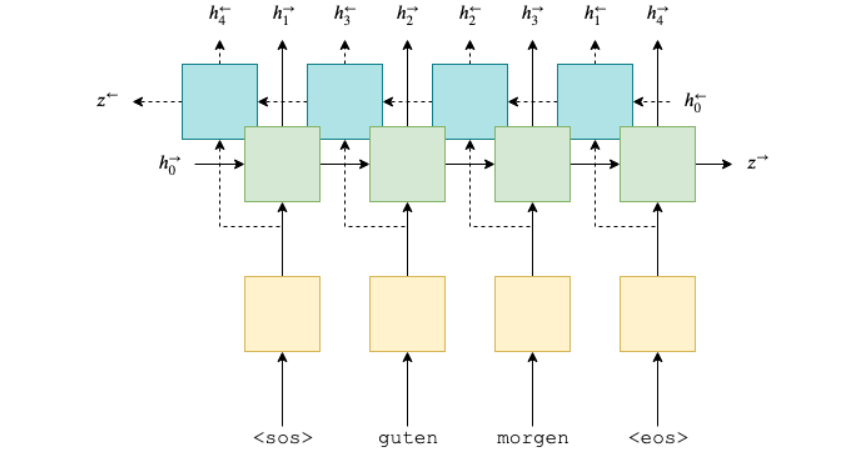
\includegraphics[width=\linewidth]{encoder}
    \caption{Kodetzailea}
    \label{fig:encoder}
\end{figure}

\subsubsection{Atentzioa}

Atentzio geruzak deskodetzailearen aurreko ezkutuko egoera hartuko du, $s_{t-1}$, eta kodetzailearen ezkutuko aurreranzko eta atzeranzko egoera guztiak, $H$. Geruzak atentzio bektorea itzuliko du, $a_t$, iturburu esaldiaren luzera duen bektorea. Elementu bakoitza 0 eta 1 artekoa izango da eta bektore osoaren batura 1. Bektore honek adierazten du sarrerako esaldiko zer hitzi jarri behar diogun arreta hurrengo hitza aurreikusteko, $\hat{y}_{t+1}$.

Lehenik eta behin, aurreko deskodetzaile ezkutuko egoeraren eta kodetzaile ezkutuko egoeren arteko energia kalkulatuko dugu. Honek kodetzailearen ezkutuko egoera bakoitza aurreko deskodetzaile ezkutuko egoerarekin zenbateraino bat datorren adierazten du. $E_t$ energia kalkulatuko dugu $attn$ geruza linealetik eta $\tanh$ aktibazio funtzio batetik pasatuz.

$$E_t = \tanh(\text{attn}(s_{t-1}, H))$$ 

Honek sarrerako esaldiaren luzera izatea nahi dugu. Horretarako, energia $v$ bektorearekin biderkatuko dugu. Pentsa dezakegu $v$ kodetzaileren ezkutuko egoera guztien energiaren baturaren pisuak direla. Pisu hauek adierazten digute zenbateko arreta hartu beharko genukeen token bakoitzari iturburu sekuentzian. $v$ parametroak ausaz hasieratzen dira, baina gainerako ereduarekin atzera hedapenaren bidez ikasten dira.

$$\hat{a}_t = v E_t$$

Azkenik, atentzio bektoreak murriztapenak betetzen dituela ziurtatuko dugu, $ \text{softmax}$ geruzatik igaroz.

$$a_t = \text{softmax}(\hat{a_t})$$

Adibidez, ikusi \ref{fig:attention} irudia. Hau lehen arreta bektorea kalkulatzeko da, non $s_{t-1} = s_0 = z$. Bloke berdeek ezkutuko egoerak adierazten dituzte eta atentzioaren kalkulua bloke arrosaren barruan egiten da.

\begin{figure}[ht]
    \centering
    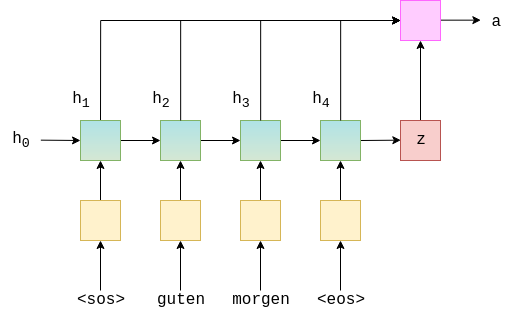
\includegraphics[width=\linewidth]{attention}
    \caption{Atentzioa}
    \label{fig:attention}
\end{figure}

\subsubsection{Deskodetzailea}
Deskodetzaileak aurretik azaldutako atentzio geruza dauka barnean. Esan bezala, aurreko ezkutuko egoera hartzen du, $s_{t-1}$, kodetzaile ezkutuko egoera guztiak, $H$, eta arreta bektorea itzultzen du, $a_t$.

Atentzio bektore hau erabiltzen dugu iturri bektore pisatua sortzeko, $w_t$, , hau da, kodetutako ezkutuko egoeren batura pisatua, $H$, pisu gisa $a_t$ erabiliz.

$$w_t = a_t H$$

Sarrerako hitzaren embeddinga, $d(y_t)$, iturburuko bektore pisatua, $w_t$, eta deskodetzailearen aurreko ezkutuko egoera, $s_{t-1}$, RNNra pasatzen dira, $d(y_t)$ eta $w_t$ elkarrekin kateatuz.

$$s_t = \text{DecoderGRU}(d(y_t), w_t, s_{t-1})$$

Ondoren, $d(y_t)$, $w_t$ eta $s_t$ kateatu eta geruza lineal batetik pasatzen dira, $f$, irteerako esaldiko hurrengo hitza aurreikusteko, $\hat{y}_{t+1}$.

$$\hat{y}_{t+1} = f(d(y_t), w_t, s_t)$$

Ikusi \ref{fig:decoder} irudian adibideko lehen hiztaren deskodeketa. Bloke berdeek $H$ itzultzen duten aurreranko eta atzeranzko RNNak adierazten dituzte. Bloke gorriak testuinguru bektorea adierazten du, $z = h_T = \tanh(g(h^\rightarrow_T,h^\leftarrow_T)) = \tanh(g(z^\rightarrow, z^\leftarrow)) = s_0$. Bloke moreak $f$ geruza lineala adierazten du, $\hat{y}_{t+1}$ itzultzen duena. Bloke laranjak batura pisatuaren kalkulua egiten du, $w_t$, $H$ eta $a_t$ erabiliz.

\begin{figure}[ht]
    \centering
    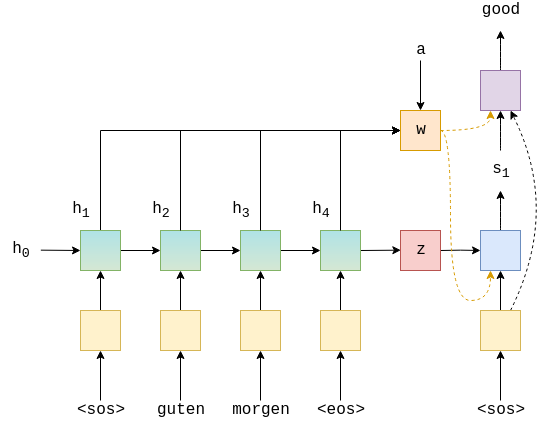
\includegraphics[width=\linewidth]{decoder}
    \caption{Deskodetzailea}
    \label{fig:decoder}
\end{figure}

\subsection{Entrenamendua}

Hasteko, ereduaren tamaina txikitu dugu, parametro kopurua 71 milioi ingurutik 28 milioi ingurura jaitsiz. Izan ere, bestela entrenamendu denborak oso luzeak ziren, eta pentsatu dugu ereduak konplexutasun nahikoa izango zuela erabili dugun datu kopururako. Denbora edo konputazio ahalmen handiagoa izango bagenu, eredu konplexuagoa eta datu gehiago erabiltzea hobe izango litzateke.

Entrenamenduko pausoetan ere aldaketak egin ditugu. Alde batetik, balidazioko pausoa gehitu dugu epoch bakoitzean. Bestetik, epoch bakoitzeko galera eta perplexitatea gorde ditugu ondoren grafikak atera ahal izateko. Amaitzeko, ereduen checkpoint-ak egin ditugu epoch bakoitzean, entrenamendua geratzen bada aurrerago jarraitu ahal izateko. Horretarako, ereduaren egoeraz gain optimizatzailearen egoera, epoch zenbakia eta aurretik esandako galera eta perplexitate balioak gorde ditugu. Izan ere, entrenatzeko denbora asko behar zen, eta oso zaila da dena segidan egitea.

Euskarako eredua 50 epoch entrenatu dugu 500.000 daturekin. Ikusi \ref{fig:loss} eta \ref{fig:ppl} irudiak. Ikasketa kurba nahiko arraroa atera zaigu kasu honetan, salto arraroak daude checkpoint-ak kargatu ditugun lekuetan. Puntu horietan balidazioko galera jaitsi egiten da, eta entrenamendukoa igo. Hala ere, argi dago eredua overfitting egiten ari dela, entrenamenduko galera jaisten ari da eta balidaziokoa igotzen.

\begin{figure}[ht]
    \centering
    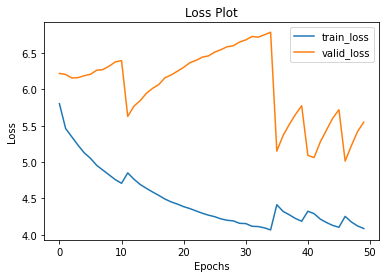
\includegraphics[width=\linewidth]{loss}
    \caption{Euskarazko ereduaren Loss}
    \label{fig:loss}
\end{figure}

\begin{figure}[ht]
    \centering
    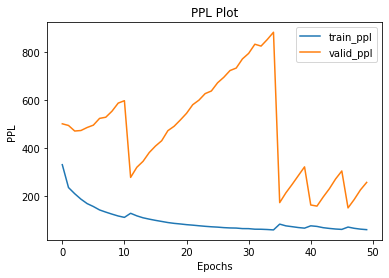
\includegraphics[width=\linewidth]{ppl}
    \caption{Euskarazko ereduaren PPL}
    \label{fig:ppl}
\end{figure}

Testuingurudun eredua 50 epoch entrenatu dugu 100.000 daturekin. Ikusi \ref{fig:loss_context} eta \ref{fig:ppl_context} irudiak. Kasu honetan ikasketa kurba normalagoa da. Izan ere, ez dugu checkpoint-ik erabili beharrik izan, entrenamendu denbora laburragoa zelako. Aurreko ereduak bezala overfitting egiten ari da. Datu gutxiago erabiltzen direnez, entrenamenduko galera azkarrago jaisten da, baina aldi berean balidaziokoa azkarrago igotzen da.

\begin{figure}[ht]
    \centering
    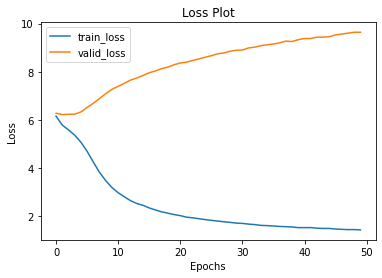
\includegraphics[width=\linewidth]{loss_context}
    \caption{Testuingurudun ereduaren Loss}
    \label{fig:loss_context}
\end{figure}

\begin{figure}[ht]
    \centering
    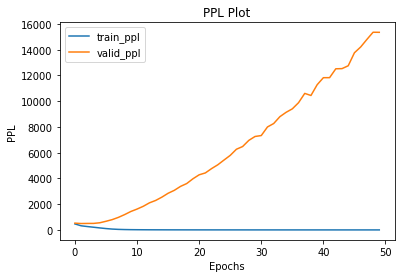
\includegraphics[width=\linewidth]{ppl_context}
    \caption{Testuingurudun ereduaren PPL}
    \label{fig:ppl_context}
\end{figure}

\subsection{Inferentzia}
Inferentziarako erabiltzailearen esaldia pasatzen zaio kodetzaileari. Guk esaldi hau garbitzea eta tokenizatzea erabaki dugu, entrenamenduko fitxategiarekin egiten den bezala. Testuingurudun ereduan sarrerako esaldiari testuingurua gehitu behar zaio. Horretarako, nahikoa da aurreko txandako balioa gordetzea eta hurrengo txandan ereduari pasatzea.

Ondoren, kodetzailearen emaitza eta hasierako tokena deskodetzaileari pasatzen zaizkio. Deskodetzailea erabiliz banaka hitz berriak sortu beharko ditugu. Baina deskodetzaileak itzultzen duena probabilitate distribuzio bat denez, hainbat estrategia daude hitza aukeratzeko.

Gure kasuan 3 greedy deskodeketa estrategia probatu ditugu: top1, topk eta multinomial. Top1 estrategiak beti token probableena aukeratuko du. Beraz, sarrera bererako beti irteera bera itzultzen du. Topk estrategiak k probableenen artean ausaz aukeratzen du. Multinomial estrategiak probabilitate distribuziotik lagintzen ditu tokenak. Tenperatura parametroa handitu daiteke probabilitate distribuzioa leuntzeko. Horrela, tenperatura baxua bada, zailagoa izango da probabilitate txikia duten tokenak aukeratzea.

\subsection{Telegrameko txatbota}

Txatbot bat, adimen artifiziala (AA) erabilita, erabiltzaile batekin lengoaia naturaleko elkarrizketa bat simulatu dezakeen aplikazio bat da.
Gure kasuan, Telegrameko API-a erabiliz, txatbot bat sortu dugu, \href{https://t.me/HPDialbot}{Dialbot}. Txatbot honek, erabiltzaileak idatzitako mezua jaso eta aurrez entrenatu ditugun ereduak erabiliz, erabiltzaileari erantzuten dio.
Txatbotak hainbat ezarpen desberdin ditu, hizkuntza zein aurreko azpisekzioan azaldutako deskodeketa estrategia bat aukeratu daiteke. Horretarako hainbat komando desberdin daude.

\begin{figure}
    \centering
    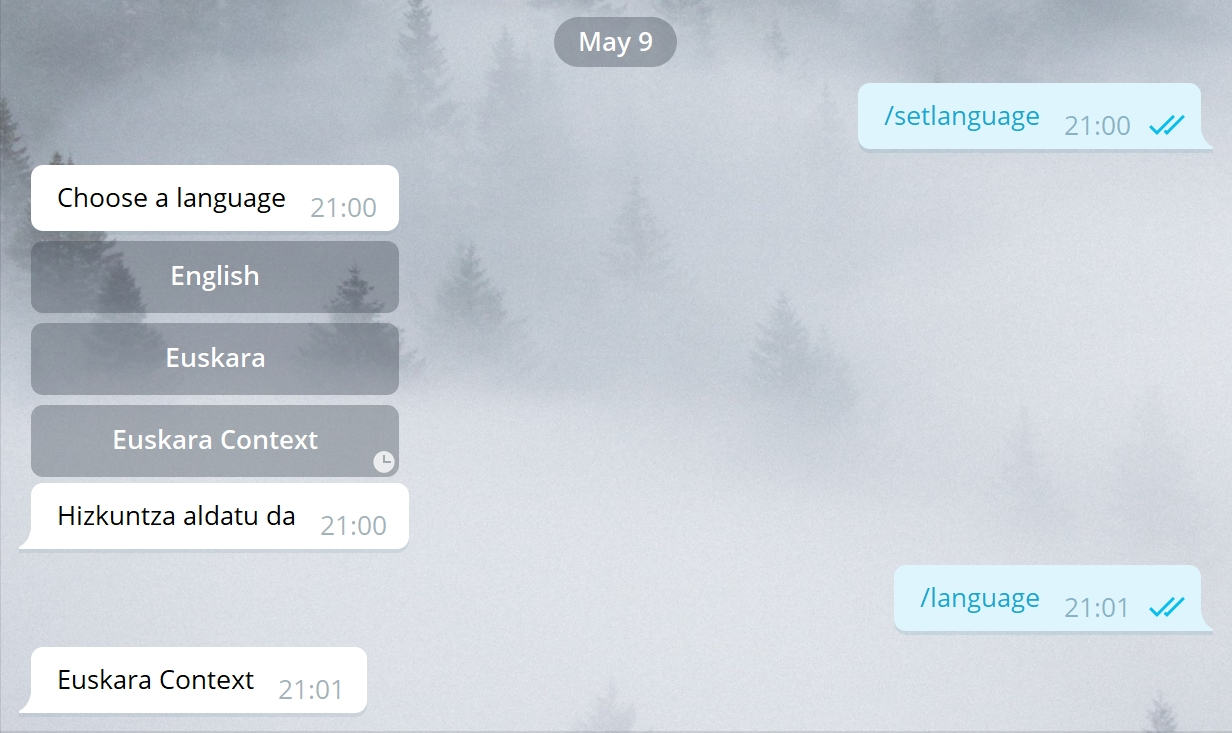
\includegraphics[width=\linewidth]{images/bot_language.jpg}
    \caption{Hizkuntza aldatu telegrameko txatbotean}
    \label{fig:hizkuntza}
\end{figure}

\begin{figure}
    \centering
    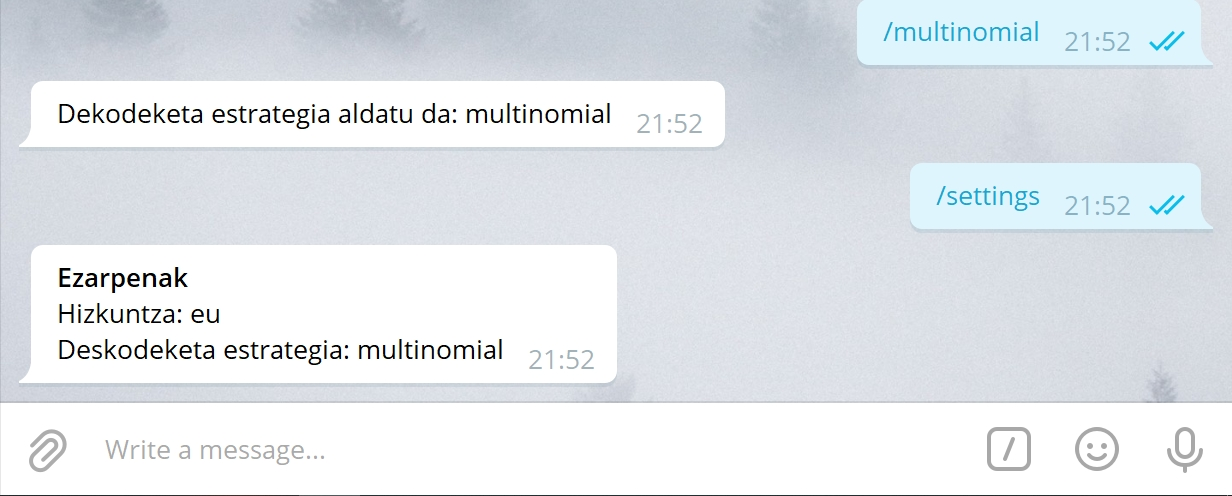
\includegraphics[width=\linewidth]{images/bot_decoding.jpg}
    \caption{Deskodeketa aldatu telegrameko txatbotean}
    \label{fig:hizkuntza2}
\end{figure}

Alde batetik lengoaiarekin zerikusia duten komandoak daude:
\begin{enumerate}
    \item \textbf{\textbackslash eu} komandoak txatbotaren hizkuntza euskarara aldatzen du, hau da, euskarako eredua erabiliko du elkarrizketan.
    \item \textbf{\textbackslash en} komandoak txatbotaren hizkuntza ingelesera aldatzen du, hau da, ingeleseko eredua erabiliko du elkarrizketan.
    \item \textbf{\textbackslash context} komandoak ere txatbotaren hizkuntza euskarara aldatzen du, baina, testuingurudun euskarako eredua erabiliko du elkarrizketan.
    \item \textbf{\textbackslash setlanguage} komandoak botoi bidez hizkuntza aldatzeko aukera ematen du. \ref{fig:hizkuntza} irudian ikus daiteke adibide bat.
    \item \textbf{\textbackslash language} komandoak txatbotaren uneko hizkuntza itzultzen du. \ref{fig:hizkuntza} irudian ikus daiteke adibide bat.
\end{enumerate}

Bestalde, deskodeketa estrategiarekin lotuta dauden komandoak daude:
\begin{enumerate}
   \item \textbf{\textbackslash top1} komandoak txatbotaren deskodeketa 
 estrategia top1-era aldatzen du.
    \item \textbf{\textbackslash topk} komandoak txatbotaren deskodeketa estrategia topk-ra aldatzen du.
    \item \textbf{\textbackslash multinomial} komandoak txatbotaren deskodeketa estrategia multinomialera aldatzen du.  \ref{fig:hizkuntza2} irudian ikus daiteke adibide bat.
    \item \textbf{\textbackslash setdecoding} komandoak botoi bidez deskodeketa estrategia aldatzeko aukera ematen du.
    \item \textbf{\textbackslash decoding} komandoak txatbotaren uneko deskodeketa estrategia itzultzen du.
\end{enumerate}

Amaitzeko, beste bi komando ere badaude:

\begin{enumerate}
    \item \textbf{\textbackslash settings} komandoak uneko hizkuntza eta deskodeketa estrategia itzultzen ditu.\ref{fig:hizkuntza2} irudian ikus daiteke adibide bat.
    \item \textbf{\textbackslash help} komandoak komando guztien lista itzultzen du.

\end{enumerate}

\section{Emaitzak}

\subsection{Inferentzia}

Ingeleseko ereduarekin hainbat proba egin ditugu deskodeketa estrategia desberdinekin eta k eta tenperatura desberdinekin. Orokorrean ikusi dugu k eta tenperatura handitzean emaitza arraroagoak lortzen direla. Beste bi ereduetarako ere 3 aukerak probatu ditugu, baina k eta tenperatura defektuzko balioak erabiliz. Egindako probekin esango genuke eredu onena ingelesekoa dela, ondoren testuingurudun eredua eta azkenik testuingururik gabea.

Bestalde, deskodeketa estrategi desberdinekin lortutako emaitzen adibide batzuk jarraian ikus daitezke.

Deskodeketa multinomiala:
\begin{verbatim}
   - Hello, how are you?
   + i ' good and you  ?
   
   - Hello, how are you?
   +i 'm great .! 
    i am a tour student.
\end{verbatim}

Topk deskodeketa:
\begin{verbatim}
   - Hello, how are you?
   + great how are you  like
   
   - Hello, how are you?
   + ok just so what kind 
     hows new shoes ? i

\end{verbatim}

Top1 deskodeketa:
\begin{verbatim}
   - Hello, how are you?
   + i 'm good great  .  
     i 'm great  .  
     what are you  ?
\end{verbatim}

Gure ustetan hoberena multinomiala da, esaldiek ia beti erabiltzailearen sarrerarekin zerikusia izateaz gain, gramatikoki zuzenak baitira. Top1 eta topk-ren artean, top1-en emaitzak topk-renak baino konsistenteagoak dira. Topk-ak sortutako erantzun askok ez dute erabiltzaileak idatzitakoarekin zerikusirik, nahiz eta beste batzutan emaitzak onargarriak izan. 

\subsection{Atentzioa}
Sortutako helburu token bakoitzaren ereduaren atentzioa erakusten duen funtzioa inplementatu dugu. Ebaluatzeko funtzioa erabiliko dugu iragarritako esaldia eta atentzioa lortzeko. Grafikoki erakusten dugu iturburuko esaldia x ardatzean eta iragarritako esaldia y ardatzean. Zenbat eta karratu argiagoa, orduan eta atentzio handiagoa eman dio ereduak iturburu-hitz horri helburu-hitz hori itzultzerakoan.

Sistema bakoitzerako adibide bana atera dugu, atentzioa nolakoa den ideia bat egiteko. Ikusi irudiak \ref{fig:attention_en}, \ref{fig:attention_eu} eta \ref{fig:attention_context}. Ingeleseko sistemaren eta beste bien artean aldea nabarmena da, dena zuria edo beltza baita. Euskarazko atentzioan gris desberdin asko daude. Atentzioetan fijatzen bagara, zaila da jakitea zenbaterainoko erabilgarria den. Itzulpenarekin konparatuta, dialogoan gutxiago laguntzen duela uste dugu. Izan ere, itzulpeneko atazan oso argi ikus daiteke atentzioa egokia al den. Baina, dialogoan sarrerarako hitzen eta irteerako hitzen lortura ez da horren zuzena.

\begin{figure}[ht]
    \centering
    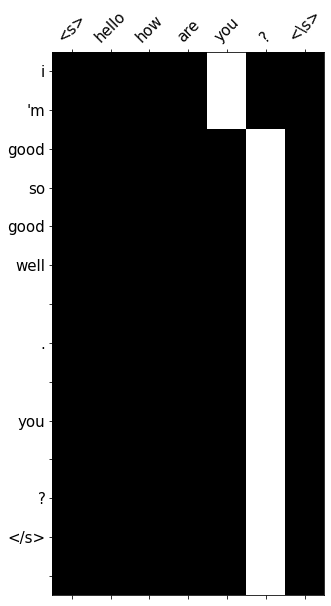
\includegraphics[width=\linewidth]{attention_en}
    \caption{Ingeleseko atentzio adibidea}
    \label{fig:attention_en}
\end{figure}

\begin{figure}[ht]
    \centering
    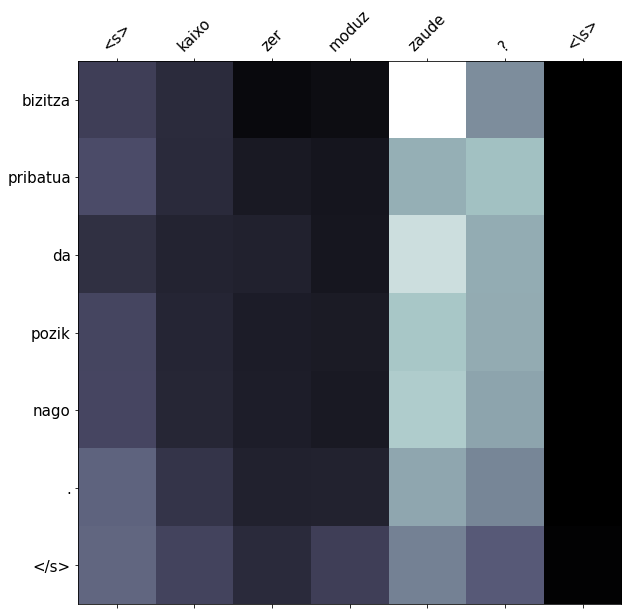
\includegraphics[width=\linewidth]{attention_eu}
    \caption{Euskararako atentzio adibidea}
    \label{fig:attention_eu}
\end{figure}

\begin{figure}[ht]
    \centering
    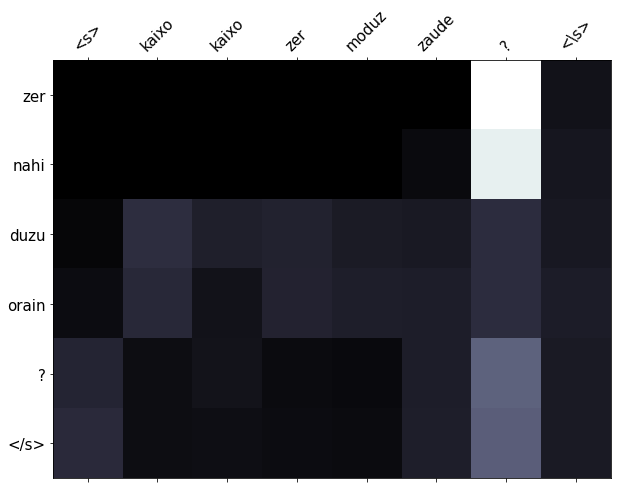
\includegraphics[width=\linewidth]{attention_context}
    \caption{Testuingurudun atentzio adibidea}
    \label{fig:attention_context}
\end{figure}

\subsection{Metrikak}

Entrenamendua amaitutakoan, ereduen hainbat metrika kalkulatu ditugu eskuzko ebaluazioaren osagarri moduan. Dialogo sistemetan ebaluazio automatikoa ez da oso esanguratsua eta errealitatean beti egiten da eskuzko ebaluazio bat gizakiekin. Hala ere, metrikak erabiltzea ez dago soberan.

Entrenatzerakoan ereduaren galera edo perplexitatea baino ez zitzaigun axola. Hala ere, itzulpenaren edo dialogoaren kalitatea neurtzeko bereziki diseinatutako metrikak daude - ezagunena BLEU da. BLEUk aurreikusitako eta benetako sekuentzien gainjartzea aztertzen du bere n-grametan. 0 eta 1 arteko zenbaki bat emango digu sekuentzia bakoitzeko, non 1-ek gainjartze perfektua dagoen esan nahi duen. Hala ere, normalean 0 eta 100 artean agertzen da. BLEU iturburu sekuentzia bakoitzeko hautagaien itzulpen anitzetarako diseinatu zen, baina datu multzo honetan iturri bakoitzeko hautagai bakarra dugu.

Datu-multzo osoaren BLEU kalkulatzeko denbora asko behar denez, bakoitzarekin 10 iterazio bakarrik egin ditugu, hau da, 640 adibide. Gainera, adibide horiek ausaz aukeratzen direnez, ez dira berdinak ebaluazio guztietan. Beraz, ondorengo emaitzak ez dira oso zehatzak, baina pentsatu dugu honekin nahikoa dela ideia bat egiteko.

Hasteko, ingeleseko entrenamenduko fitxategirako BLEU kalkulatu dugu deskodeketa estrategia desberdinak erabilita. Gainera, topk eta multinomial estrategietan k eta tenperatura parametro desberdinak probatu ditugu, nolako eragina duten jakiteko. Orokorrean, ikusi dugu k eta tenperatura handitzean emaitza okerragoak lortzen direla. Ikusi \ref{tab:decoding} taula. Bertan ikus daiteke top1 eta multinomial estrategiekin emaitza askoz hobeak lortzen direla. Eta kontuan hartuta top1 estrategiak beti emaitza bera itzultzen duela, gure ustez multinomial estrategia da onena. 

Argi geratu da deskodeketa estrategiak ere eragin handia duela azken sistemaren kalitatean. Izan ere, errealitatean baseline bezala beam search algoritmoa erabiltzen da decoding-a egiteko eta guk erabiltzen ditugun greedy estrategiak oso sinpleak dira, decoding pauso bakoitzean bide bakarra mantentzen baitute.

\begin{table}
\centering
\begin{tabular}{ |c|c| } 
    \hline
    & BLEU \\
    \hline
    Train EN Top1 & 29.78 \\ 
    Train EN Topk k=3 & 5.17 \\ 
    Train EN Topk k=7 & 1.66 \\ 
    Train EN Topk k=10 & 1.03 \\ 
    Train EN Multinomial t=0.4 & 29.85 \\ 
    Train EN Multinomial t=0.7 & 22.96 \\ 
    Train EN Multinomial t=1.0 & 15.15 \\ 
    \hline
\end{tabular}
\caption{Ingeleseko deskodeketa estrategien BLEU}
\label{tab:decoding}
\end{table}

Ondoren, multinomial estrategiarekin egin ditugu gainerako probak. Ikusi \ref{tab:metrics} taula. Sistema guztietako datuen azpimultzo bakoitzerako galera, perplexitatea eta BLEU kalkulatu ditugu. Emaitza onenak ingeleseko sistemak lortu ditu eta ondoren testuingurudun sistemak. Hori bai, esan beharra dago agian datu hauek ez direla oso esanguratsuak. Izan ere, 3 sistemak eredu eta datu desberdinekin entrenatu dira. Hala ere, idia bat egiteko behintzat balio digu.

Euskerako bi ereduen arteko aldea oso handia da. Honen arrazoia gure ustez erabilitako datu kopurua da. Testuinguruko ereduan 5 aldiz datu gutxiago erabli ditugu. Agian datu gehiegi zeuden ereduaren konplexutasuna kontuan hartuta eta horregatik kostatu zaio gehiago emaitzak hobetzea testuingururik gabeko ereduari. Ez dugu uste testuinguru sinple hau gehitzeak ereduari abantaila handirik ematen dionik.

Emaitzetan harritu gaitu eredu bererako datu-multzoan artean ia alderik ez egoteak. Honen arrazoietako bat izan daiteke entrenamendu garaian egiten den teacher forcing-a, baina horrekin bakarrik ezin daiteke azaldu. Datu-multzo desberdinekin probak egitearen helburua zen ikustea zenbateko aldea dagoen entrenamenduko eta balidazioko puntuazioen artean. Entrenatzen ari ginen bitartean balidazioko emaitzak entremendukoak bana askoz txarragoak ziren. Epoch gehiago egin ahala entrenamenduko galera jaitsi egiten zen, eta balidaziokoa igo, hau da, eredua overfitting egiten ari zen.

\begin{table}
\centering
\begin{tabular}{ |c|c|c|c| } 
    \hline
    & Loss & PPL & BLEU \\
    \hline
    Train EN & 1.686 & 5.400 & 29.85 \\ 
    \hline
    Train EU & 4.678 & 107.558 & 4.00 \\ 
    Validation EU & 4.675 & 107.263 & 1.53 \\ 
    Test EU & 4.689 & 108.763 & 2.20 \\ 
    \hline
    Train Context & 2.892 & 18.024 & 24.29 \\ 
    Validation Context & 2.880 & 17.809 & 25.21 \\ 
    Test Context & 2.882 & 17.853 & 24.18 \\ 
    \hline
\end{tabular}
\caption{Ereduen metrikak: galera, perplexitatea eta BLEU}
\label{tab:metrics}
\end{table}

\section{Ondorioak}
Lan honetan dialogoa itzulpen automatikoko ataza bat bezala definitu dugu. Esan bezala, aukera hau ez da optimoa sinplifikazio handi bat baita. Beraz, hasieratik mugatuta geunden eredu mota dela eta. Horrez gain, argi geratu da datuek duten garrantzia. Ingeleseko sistema entrenatzeko, pelikulen azpitituluak erabili beharrean elkarrizketak erabili ziren. Azkenengo hauek askoz aproposagoak dira ataza honetarako eta emaitzek garbi islatzen dute hori. 

Hala ere, esperimentu interesgarriak egiteko aukera eman digu proiektuak. Entrenatutako ereduen emaitzak ez dira horren txarrak izan, ereduak euskaraz erantzuten ikasi du. Ingeleseko ereduaren arkitektura ulertu dugu eta euskerazko ereduak entrenatu ditugu arkitektura berarekin. Eredu eta deskodeketa estrategia desberdinak ulertu eta konparatu ditugu. Bukatzeko, sistema guztia telegrameko bot bezala funtzionatzeko egokitzen ere ikasi dugu.

\bibliography{dialbot}
\bibliographystyle{acl_natbib}

\end{document}

